% Figure from MATH 591 notes, section 7. Compile with the notes preamble.
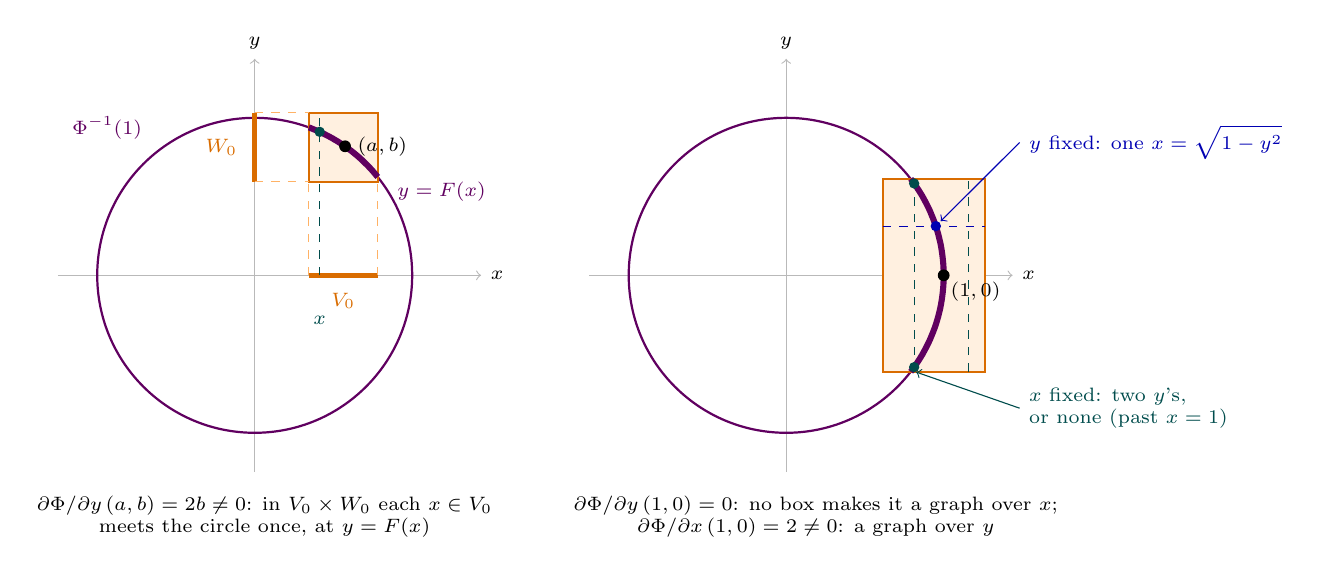
\begin{tikzpicture}[scale=1.25, font=\scriptsize]
\draw[->, gray!55] (-2,0) -- (2.3,0) node[right, text=black] {$x$};
\draw[->, gray!55] (0,-2.0) -- (0,2.2) node[above, text=black] {$y$};
\draw[violet!75!black, thick] (0,0) circle (1.6);
\draw[->, gray!55] (3.4,0) -- (7.7,0) node[right, text=black] {$x$};
\draw[->, gray!55] (5.4,-2.0) -- (5.4,2.2) node[above, text=black] {$y$};
\draw[violet!75!black, thick] (5.4,0) circle (1.6);
\fill[orange!12] (0.55,0.95) rectangle (1.25,1.65);
\draw[orange!85!black, thick] (0.55,0.95) rectangle (1.25,1.65);
\draw[violet!75!black, line width=2.2pt] plot coordinates {(0.55,1.502) (0.568,1.496) (0.585,1.489) (0.603,1.482) (0.62,1.475) (0.638,1.468) (0.655,1.46) (0.672,1.452) (0.69,1.444) (0.708,1.435) (0.725,1.426) (0.743,1.417) (0.76,1.408) (0.778,1.398) (0.795,1.389) (0.812,1.378) (0.83,1.368) (0.848,1.357) (0.865,1.346) (0.883,1.335) (0.9,1.323) (0.917,1.311) (0.935,1.298) (0.953,1.286) (0.97,1.272) (0.988,1.259) (1.005,1.245) (1.022,1.231) (1.04,1.216) (1.058,1.201) (1.075,1.185) (1.093,1.169) (1.11,1.152) (1.127,1.135) (1.145,1.118) (1.163,1.099) (1.18,1.081) (1.198,1.061) (1.215,1.041) (1.232,1.02) (1.25,0.999)};
\draw[orange!85!black, line width=2pt] (0.55,0) -- (1.25,0) node[midway, below=2pt] {$V_0$};
\draw[orange!85!black, line width=2pt] (0,0.95) -- (0,1.65) node[midway, left=2pt] {$W_0$};
\draw[orange!60, dashed] (0.55,0) -- (0.55,0.95); \draw[orange!60, dashed] (1.25,0) -- (1.25,0.95);
\draw[orange!60, dashed] (0,0.95) -- (0.55,0.95); \draw[orange!60, dashed] (0,1.65) -- (0.55,1.65);
\draw[teal!60!black, dashed] (0.66,0) -- (0.66,1.65);
\fill[teal!60!black] (0.66,1.458) circle (1.5pt);
\node[teal!60!black, below] at (0.66,-0.32) {$x$};
\fill (0.918,1.311) circle (1.7pt) node[right=1pt] {$(a,b)$};
\node[violet!75!black, anchor=west] at (1.35,0.85) {$y = F(x)$};
\node[violet!75!black] at (-1.5,1.5) {$\Phi^{-1}(1)$};
\node[align=center] at (0.1,-2.45) {$\partial\Phi/\partial y\,(a,b) = 2b \neq 0$: in $V_0 \times W_0$ each $x \in V_0$\\ meets the circle once, at $y = F(x)$};
\fill[orange!12] (6.38,-0.98) rectangle (7.42,0.98);
\draw[orange!85!black, thick] (6.38,-0.98) rectangle (7.42,0.98);
\draw[violet!75!black, line width=2.2pt] plot coordinates {(6.665,-0.98) (6.69,-0.946) (6.715,-0.912) (6.738,-0.877) (6.761,-0.841) (6.783,-0.805) (6.803,-0.768) (6.823,-0.731) (6.842,-0.693) (6.86,-0.655) (6.876,-0.616) (6.892,-0.577) (6.907,-0.538) (6.921,-0.498) (6.933,-0.458) (6.945,-0.417) (6.955,-0.376) (6.965,-0.335) (6.973,-0.294) (6.98,-0.252) (6.986,-0.21) (6.991,-0.168) (6.995,-0.126) (6.998,-0.084) (6.999,-0.042) (7,0) (6.999,0.042) (6.998,0.084) (6.995,0.126) (6.991,0.168) (6.986,0.21) (6.98,0.252) (6.973,0.294) (6.965,0.335) (6.955,0.376) (6.945,0.417) (6.933,0.458) (6.921,0.498) (6.907,0.538) (6.892,0.577) (6.876,0.616) (6.86,0.655) (6.842,0.693) (6.823,0.731) (6.803,0.768) (6.783,0.805) (6.761,0.841) (6.738,0.877) (6.715,0.912) (6.69,0.946) (6.665,0.98)};
\draw[teal!60!black, dashed] (6.7,-0.98) -- (6.7,0.98);
\fill[teal!60!black] (6.7,0.933) circle (1.5pt); \fill[teal!60!black] (6.7,-0.933) circle (1.5pt);
\draw[teal!60!black, dashed] (7.25,-0.98) -- (7.25,0.98);
\draw[blue!70!black, dashed] (6.38,0.5) -- (7.42,0.5);
\fill[blue!70!black] (6.92,0.5) circle (1.5pt);
\fill (7,0) circle (1.7pt) node[below right=-1pt] {$(1,0)$};
\node[teal!60!black, anchor=west, align=left] (T) at (7.77,-1.35) {$x$ fixed: two $y$'s,\\ or none (past $x = 1$)};
\draw[teal!60!black, ->] (T.west) -- (6.72,-0.983);
\node[blue!70!black, anchor=west] (B) at (7.77,1.35) {$y$ fixed: one $x = \sqrt{1-y^2}$};
\draw[blue!70!black, ->] (B.west) -- (6.97,0.55);
\node[align=center] at (5.7,-2.45) {$\partial\Phi/\partial y\,(1,0) = 0$: no box makes it a graph over $x$;\\ $\partial\Phi/\partial x\,(1,0) = 2 \neq 0$: a graph over $y$};
\end{tikzpicture}
